%%%%%%%%%%%%%%%%%%%%%%%%%%%%%%%%%%%%%%%%%%%%%%%%%%%%%%%%%%%%%%%%%%%%%%%%%%%%%%%%
%2345678901234567890123456789012345678901234567890123456789012345678901234567890
%        1         2         3         4         5         6         7         8
\documentclass[letterpaper, 10 pt, conference]{ieeeconf}  % Comment this line out
                                                          % if you need a4paper
%\documentclass[a4paper, 10pt, conference]{ieeeconf}      % Use this line for a4

\usepackage{float}
                                                          % paper
% uso paquete bookmark para tener bien los outlines.
\usepackage{bookmark}

% Configuro el idioma.
\usepackage[utf8]{inputenc} % Importante para mantener acentos.
\usepackage[spanish, activeacute]{babel} % Requiere: texlive-lang-spanish. Por primera vez hay que ejecutar: texconfig init> log

% Paquete para poder usar acentos en $$.
\usepackage{mathtools}
%\setmathfont{XITS math}

% Para los diagramas de flujo
\usepackage{tikz}
\usetikzlibrary{shapes.geometric, arrows}

% Elementos del diagrama
\tikzstyle{startstop} = [rectangle, rounded corners, 
minimum width=6em, 
minimum height=2em,
text centered, 
draw=black, 
fill=red!30]

\tikzstyle{io} = [trapezium, 
trapezium stretches=true, % A later addition
trapezium left angle=70, 
trapezium right angle=110, 
minimum width=6em, 
minimum height=2em, text centered, 
draw=black, fill=blue!30]

\tikzstyle{block} = [rectangle, 
minimum width=8em, 
minimum height=3em, 
text centered, 
text width=7.5em, 
draw=black, 
fill=white!30]

\tikzstyle{def} = [rectangle, 
minimum width=14em, 
minimum height=3em, 
text centered, 
text width=12em, 
draw=black, 
fill=purple!30]

\tikzstyle{swap_proccess} = [rectangle, 
minimum width=8em, 
minimum height=2em, 
text centered, 
text width=8em, 
draw=black, 
fill=orange!30]

\tikzstyle{process} = [rectangle, 
minimum width=6em, 
minimum height=2em, 
text centered, 
text width=6em, 
draw=black, 
fill=orange!30]

\tikzstyle{decision} = [diamond, 
minimum width=6em, 
minimum height=6em, 
text centered, 
draw=black, 
fill=green!30]
\tikzstyle{arrow} = [thick,->,>=stealth]

\usepackage{siunitx}

% package to get \url
\usepackage{hyperref}
\hypersetup{
  colorlinks=true,
  linkcolor=magenta,
  filecolor=magenta,
  citecolor=magenta,      
  urlcolor=magenta,
}

% Graficos electrónicos
\usepackage[RPvoltages]{circuitikz}

\IEEEoverridecommandlockouts                              % This command is only
                                                          % needed if you want to
                                                          % use the \thanks command
\overrideIEEEmargins
% See the \addtolength command later in the file to balance the column lengths
% on the last page of the document

\usepackage{graphicx}
\usepackage{graphics}

% styling for matlab/octave code.
\usepackage{matlab-prettifier}
% Configuracion, con esto puede agregar ñ.
\lstset{
  literate={ñ}{{\~n}}1
}

\usepackage{listings}

% The following packages can be found on http:\\www.ctan.org
%\usepackage{graphics} % for pdf, bitmapped graphics files
%\usepackage{epsfig} % for postscript graphics files
%\usepackage{mathptmx} % assumes new font selection scheme installed
%\usepackage{times} % assumes new font selection scheme installed
\usepackage{amsmath} % assumes amsmath package installed
%\usepackage{amssymb}  % assumes amsmath package installed

\title{\LARGE \bf Entregable Trabajo Práctico N° 4}

\author{
  Tom\'as Vidal\\
  {\it Sistemas Operativos y Redes}\\
  {\it Facultad de Ingenier\'ia, UNLP, La Plata, Argentina.}\\
  {\it 28 de Noviembre, 2024.}
}                                            % <-this % stops a space


% comienzo

% INTRO


% Figura
\newcommand{\image}[2] {
  \begin{figure}[H]
    \centering
    \includegraphics[width=0.43\textwidth]{./#1.png}
    \caption{#2}
    \label{fig:#1}
  \end{figure}
}

% Codigo
% \begin{lstlisting}[style=Matlab-editor]
% % el código va aca
% dispc("HELLO WORLD");
% \end{lstlisting}

\begin{document}
\maketitle
\thispagestyle{empty}
\pagestyle{empty}

\section{Redes presentadas}
En la figura \ref{fig:red_dada} se muestra la topología de las redes que fueron asignadas. Para hacer el análisis de la misma se empleó la dirección IP asignada \textit{181.29.152.0} con CIDR\footnote{El enrutamiento entre dominios sin clases (CIDR) es un método de asignación de direcciones IP que mejora la eficiencia del enrutamiento de datos en Internet} \textit{22}.

\begin{figure}[H]
	\centering
	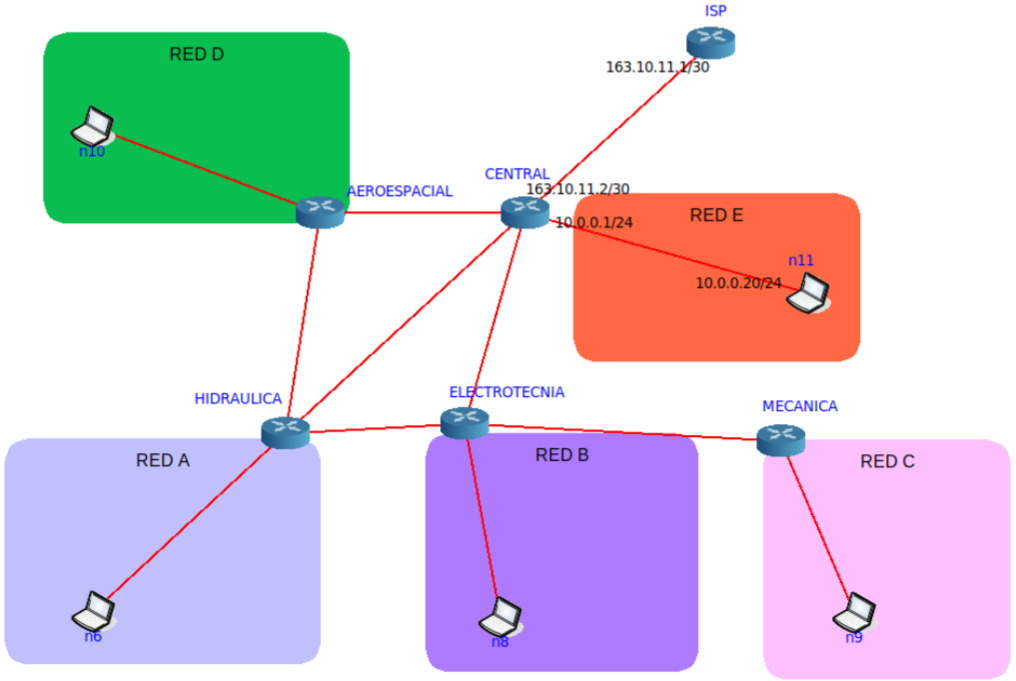
\includegraphics[width=0.43\textwidth]{./Imagenes/red_topologia.png}
	\caption{Topología de la red dada}
	\label{fig:red_dada}
\end{figure}

\subsection{Dirección IP dada}
La dirección de IP dada es \textit{181.29.148.0/22}, lo que implica que se pueden asignar un total de \textbf{1024 hosts}. Como la IP comienza con la dirección \textit{181}, la misma pertenece a la \textbf{clase B}

\subsection{Asignación de IPs}

Para hacer la asignación de IPs a las diferentes interfaces y dispositivos se hizo \textit{subnetting}\footnote{Subnetting es el proceso de dividir una red IP más grande en subredes más pequeñas, con el objetivo de optimizar el uso de direcciones IP, mejorar la seguridad y gestionar el tráfico de red de manera más eficiente.}. El proceso empleado consistió en \textit{dividir recursivamente} la IP dada en subredes más pequeñas, teniendo en cuenta las redes con mayor requerimiento de \textit{hosts}\footnote{Hosts son dispositivos conectados a una red que pueden enviar y recibir datos, como computadoras, servidores, teléfonos inteligentes, impresoras o cualquier otro equipo con una dirección IP asignada.}, es decir la \textbf{Red B}, luego la \textbf{Red A}, \textbf{D}, \textbf{C} y por último los enlaces punto a punto, para los cuales se empleó un CIDR de 30 (lo que permite optimizar la cantidad hosts).

\begin{figure}[H]
	\centering
	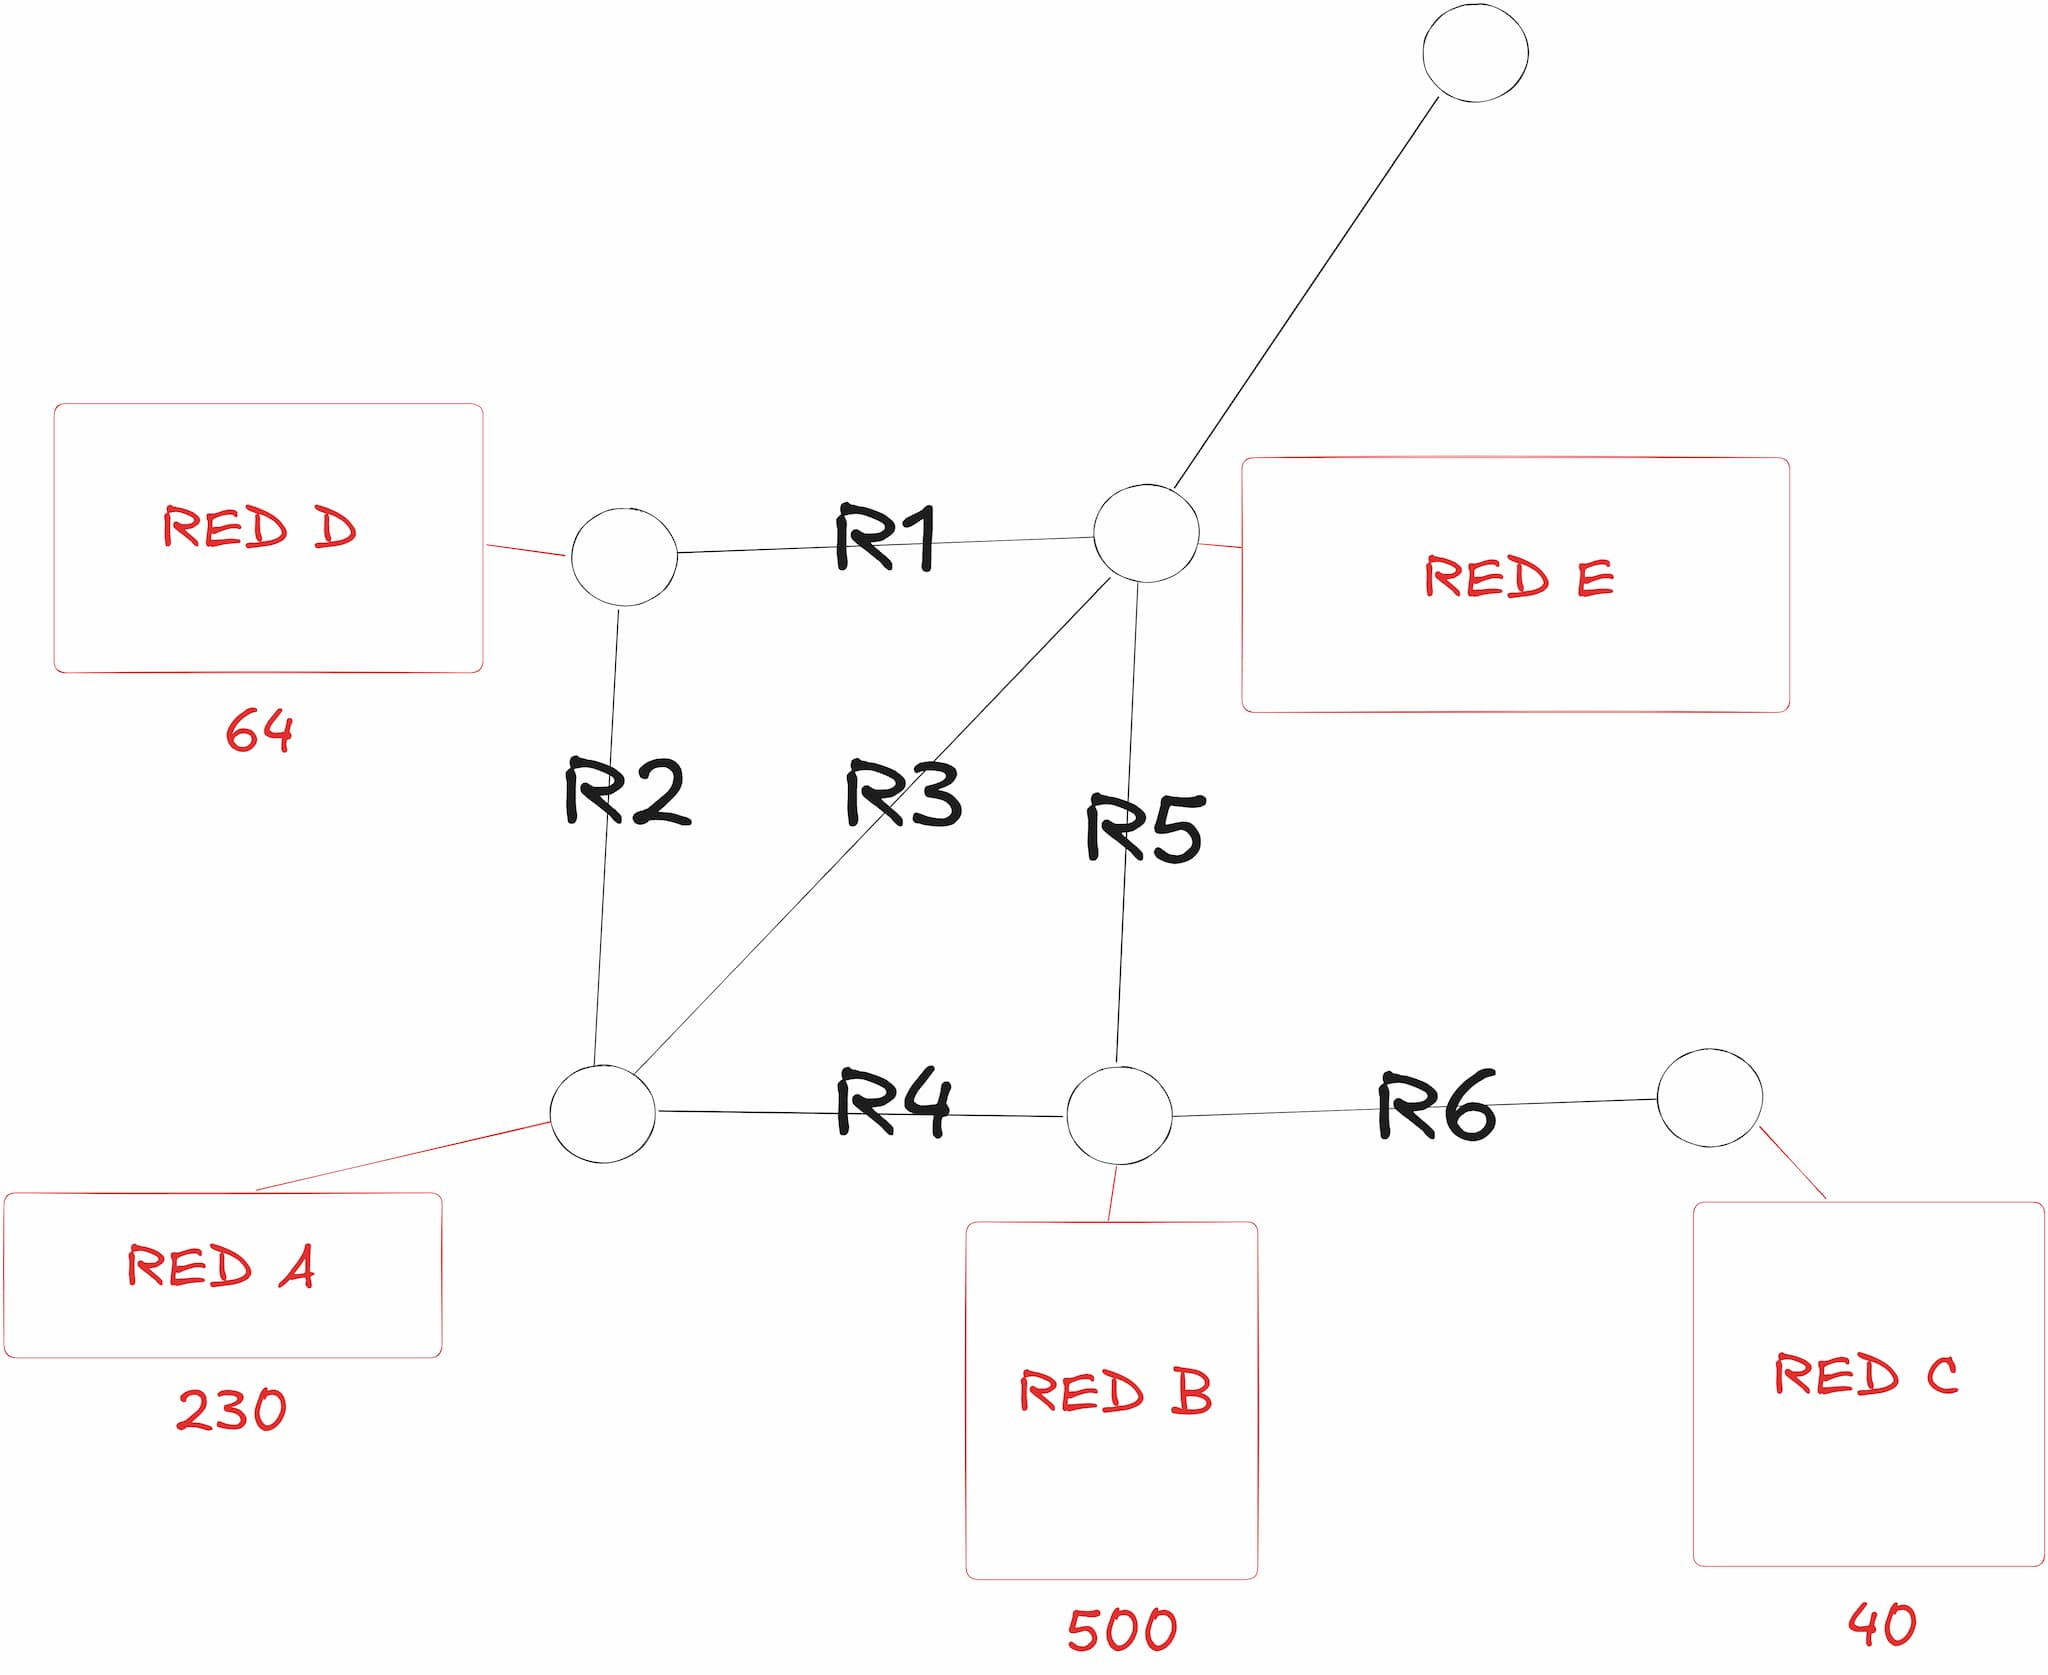
\includegraphics[width=0.43\textwidth]{./Imagenes/red_subnetting_diseno.jpg}
	\caption{Diseño de la red para hacer subnetting}
\end{figure}

\begin{figure}[H]
	\centering
	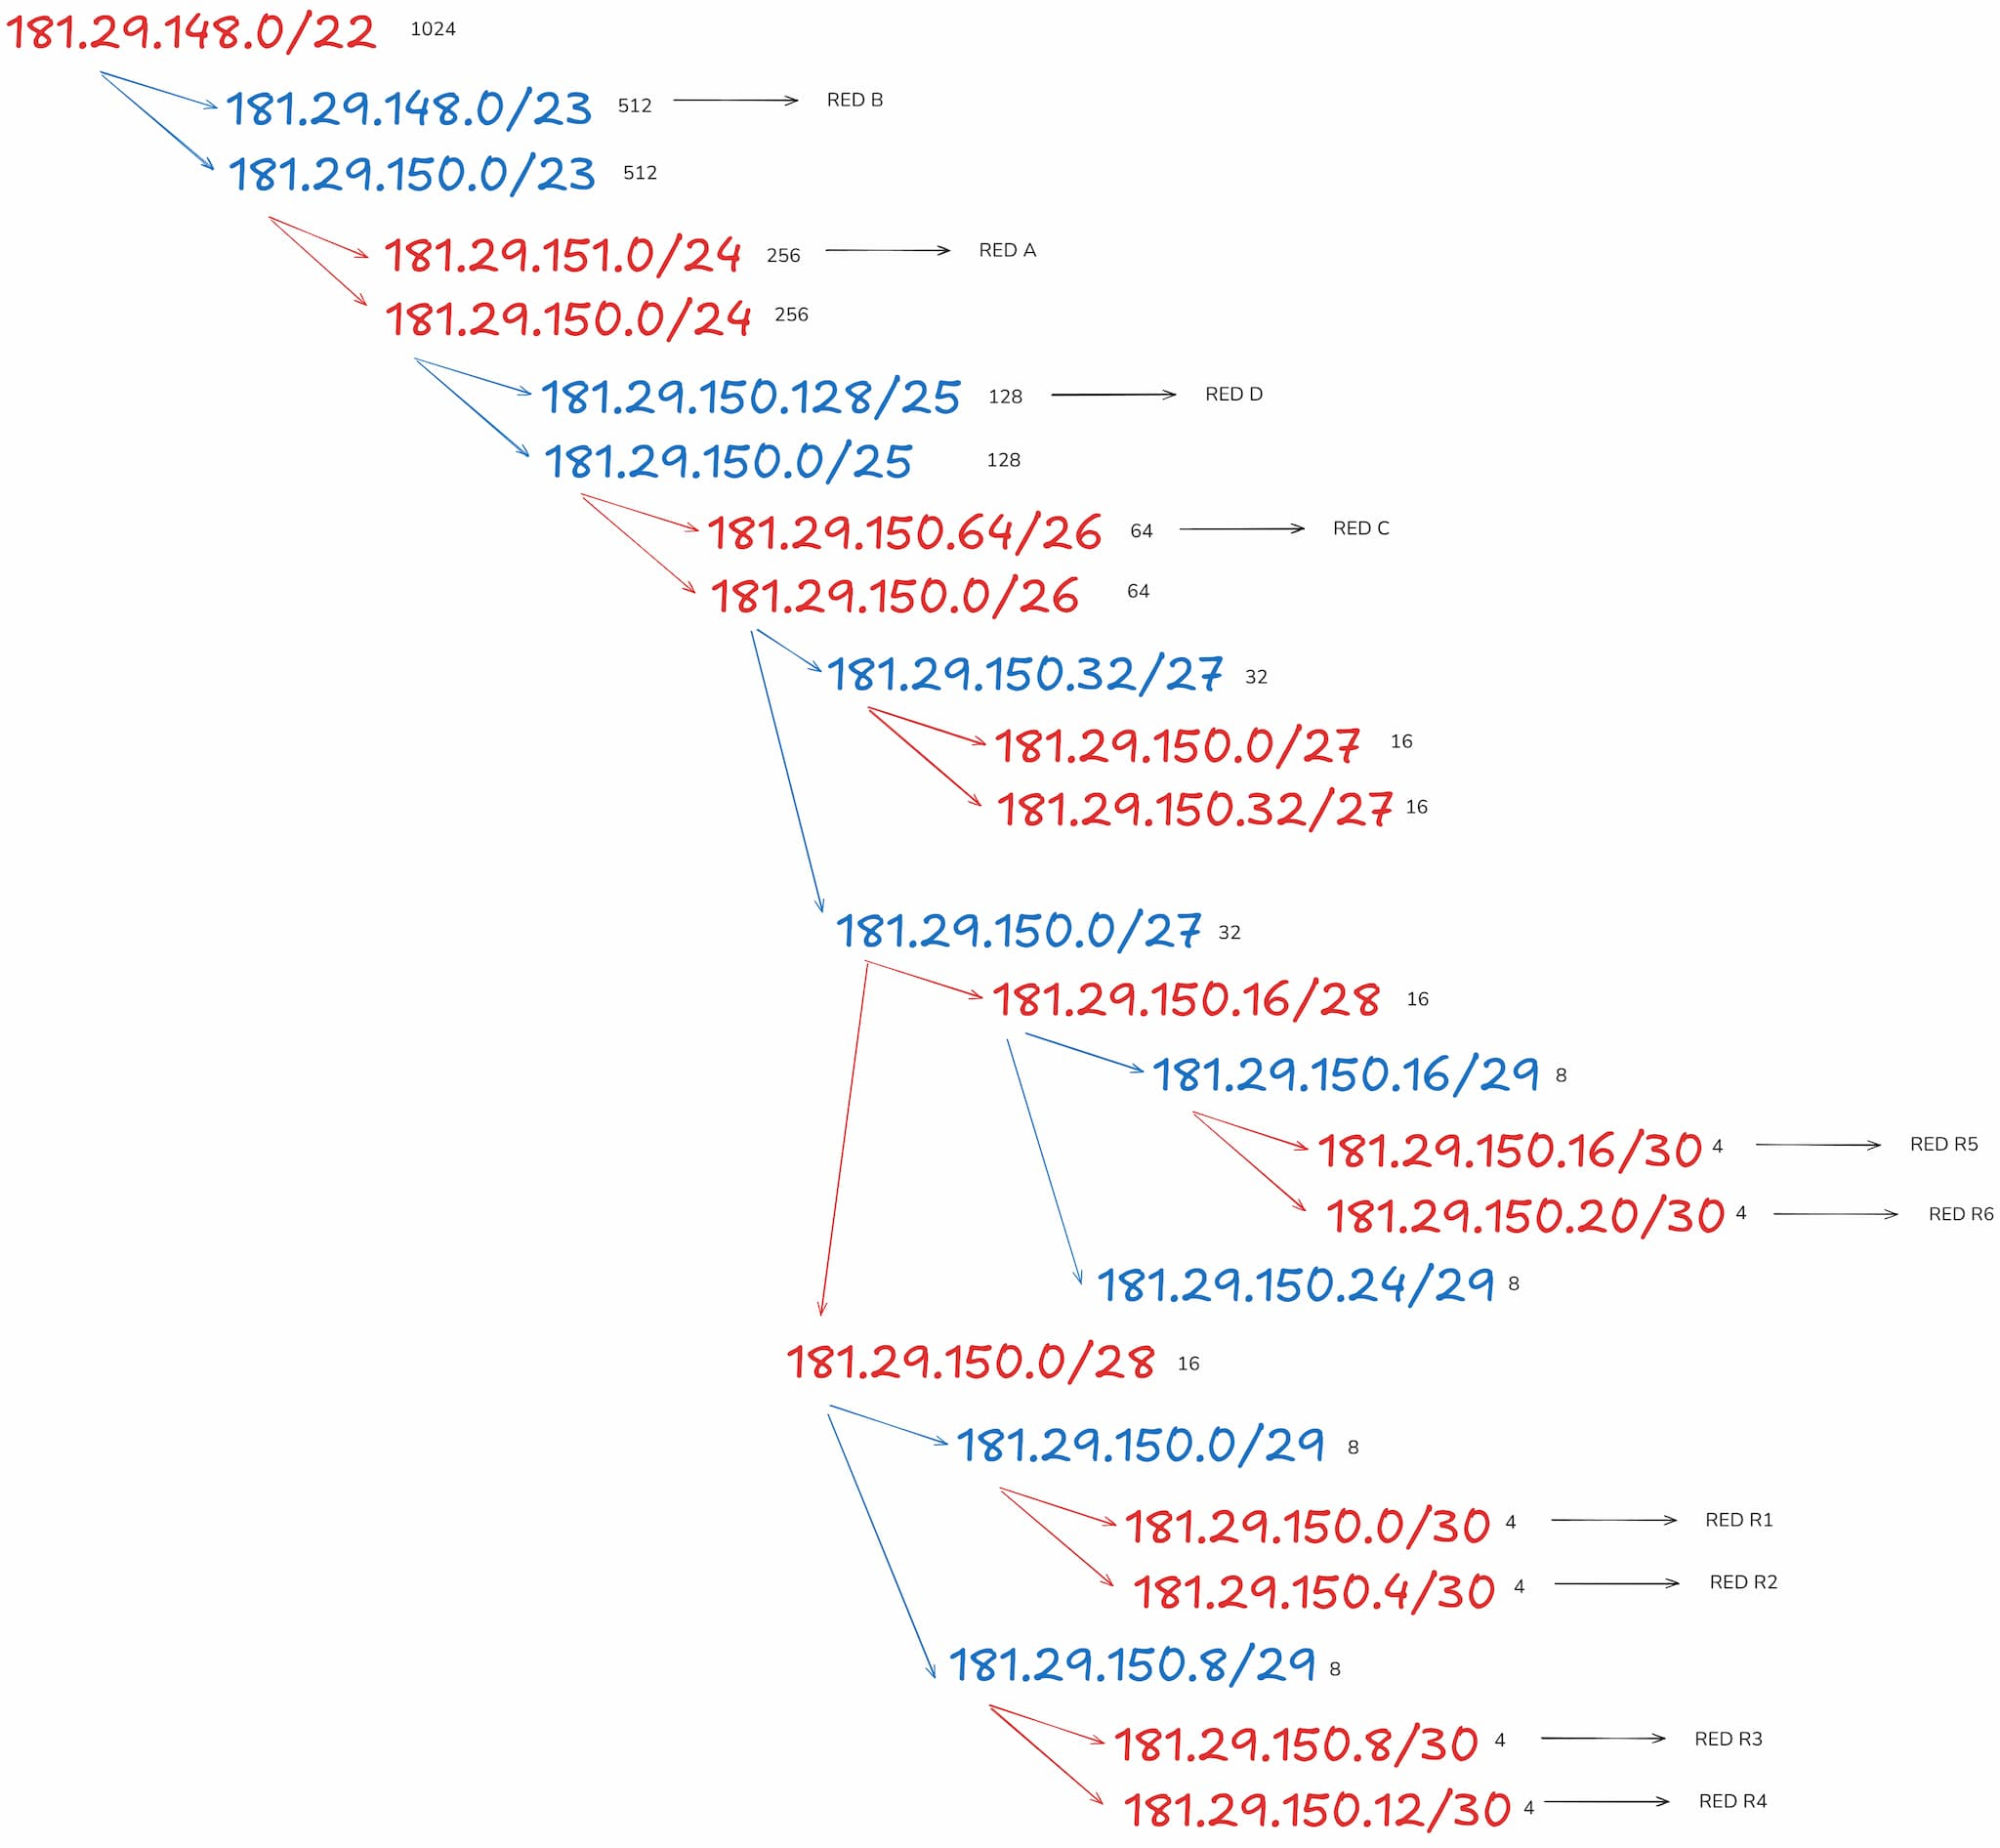
\includegraphics[width=0.43\textwidth]{./Imagenes/subnetting_total.jpg}
	\caption{Diseño subnetting de la red}
\end{figure}

\subsection{Simulación en Core Emulator}

Luego de diseñar la red y las subredes se aplicaron las IPs en el simulador Core Emulator, y para que se puedan transferir paquetes entre estas redes correctamente se hicieron enrutamientos en los diferentes \textit{routers} con los comandos:

\begin{enumerate}
	\item ip route add [GATEWAY \textit{cual}]/[CIDR] via [IP \textit{desde}] \label{cmd:add}
	\item ip route del [GATEWAY \textit{cual}]/[CIDR] via [IP \textit{desde}] \label{cmd:del}
\end{enumerate}

El comando \ref{cmd:add} se empleó para agregar redes (revelar tablas de enrutamiento), y el comando \ref{cmd:del} para eliminar una red que era incorrecta. Para guardar los cambios hechos en las tablas de enrutamiento se empleó el script provisto \textit{save}, el cual salva los cambios en el archivo ``core.txt'', además se puede emplear el comando \textit{restore core.txt} para restaurar estos cambios cuando se recarga el archivo de la topología en el Core Emulator.

Se corroboró el correcto enrutamiento de paquetes entre las redes por medio del comando \textit{traceroute}, proporcionado en una interfaz gráfica en Core Emulator, los resultados se muestran a continuación:


\begin{figure}[H]
	\centering
	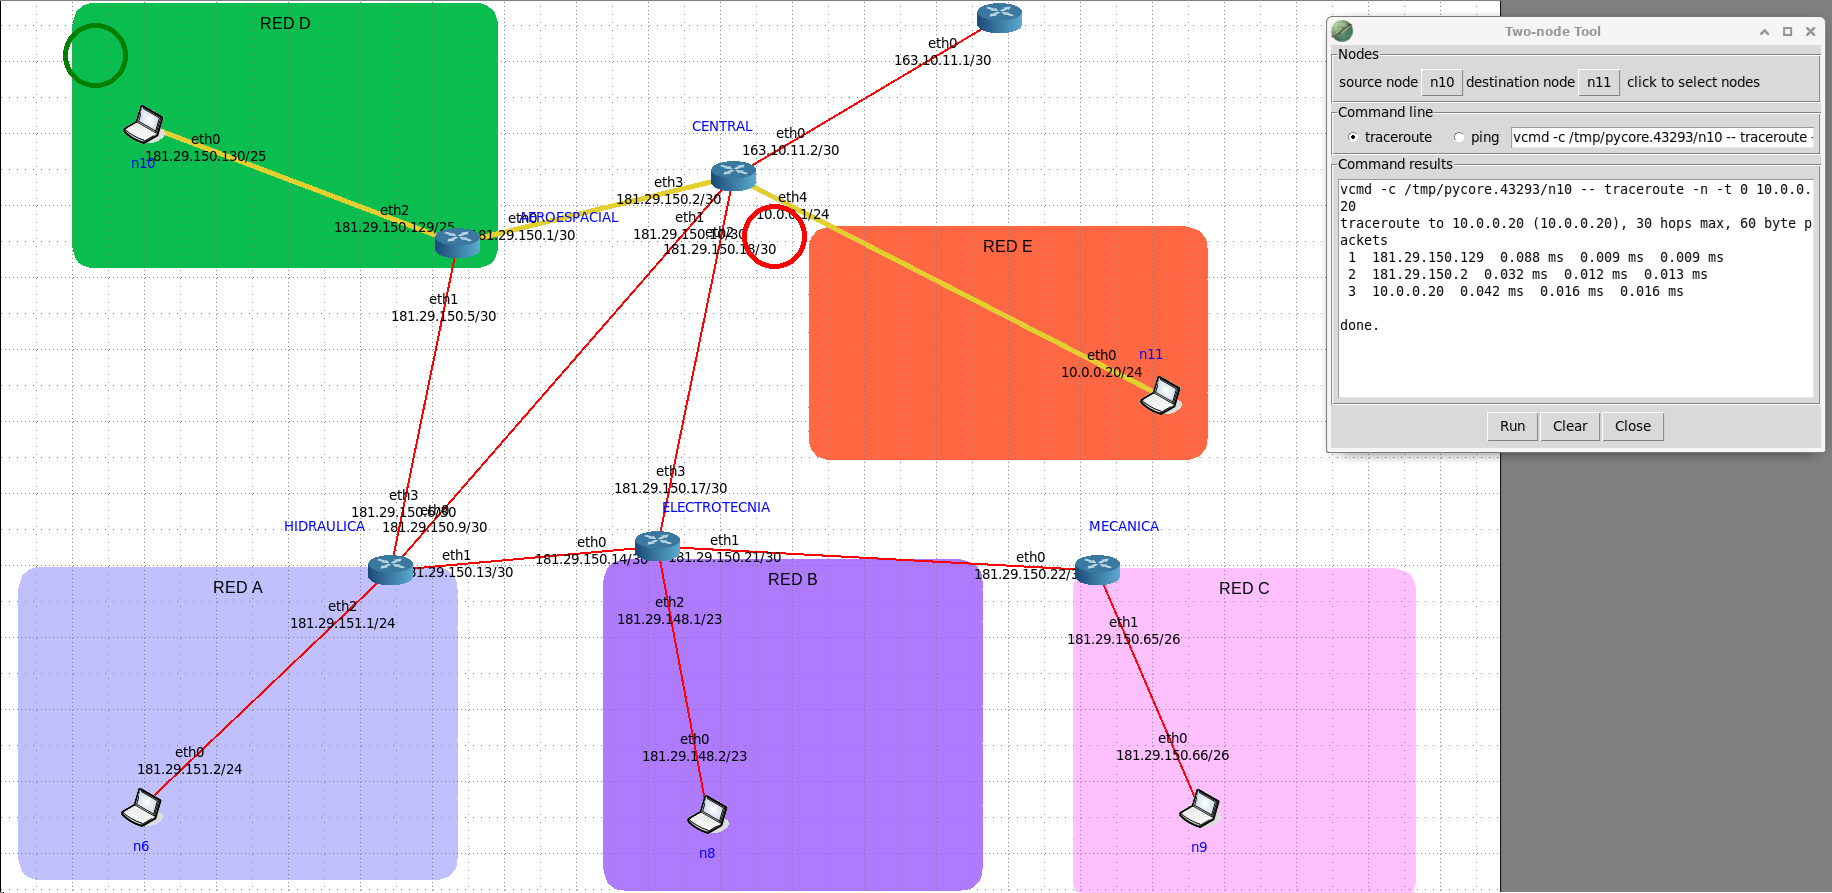
\includegraphics[width=0.43\textwidth]{./Imagenes/traceroute_1.png}
	\caption{Traceroute desde n10 a n11}
\end{figure}
\begin{figure}[H]
	\centering
	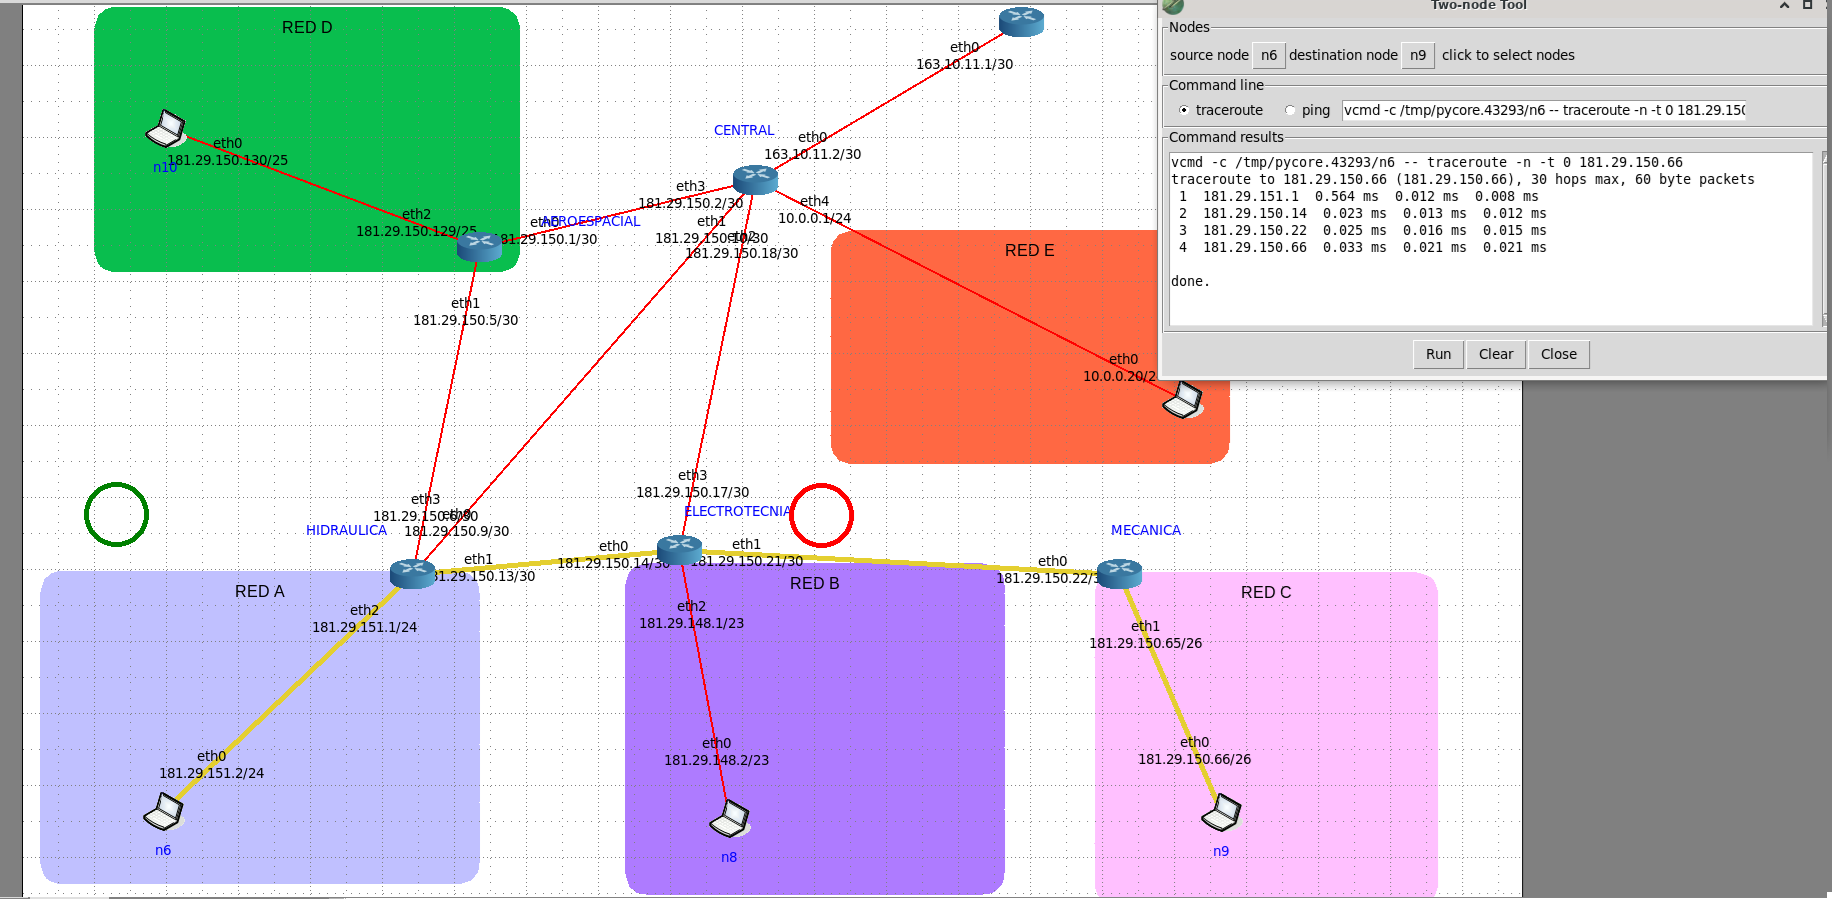
\includegraphics[width=0.43\textwidth]{./Imagenes/traceroute_2.png}
	\caption{Traceroute desde n6 a n9}
\end{figure}
\begin{figure}[H]
	\centering
	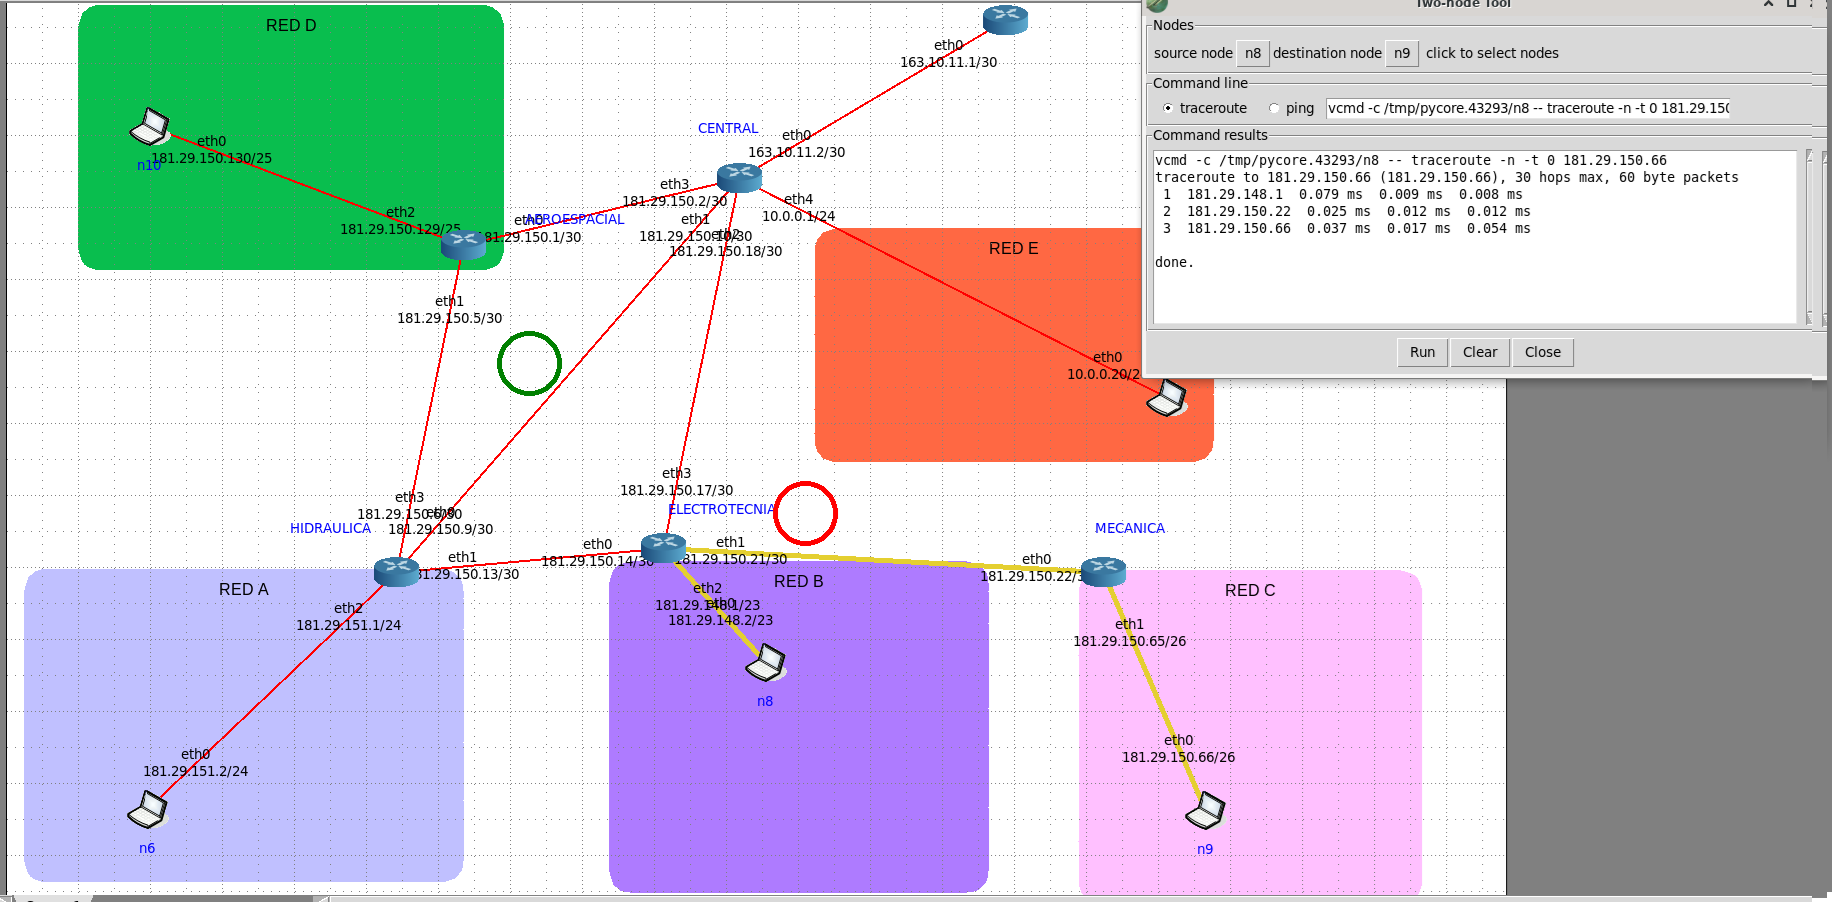
\includegraphics[width=0.43\textwidth]{./Imagenes/traceroute_3.png}
	\caption{Traceroute desde n8 a n9}
\end{figure}
\begin{figure}[H]
	\centering
	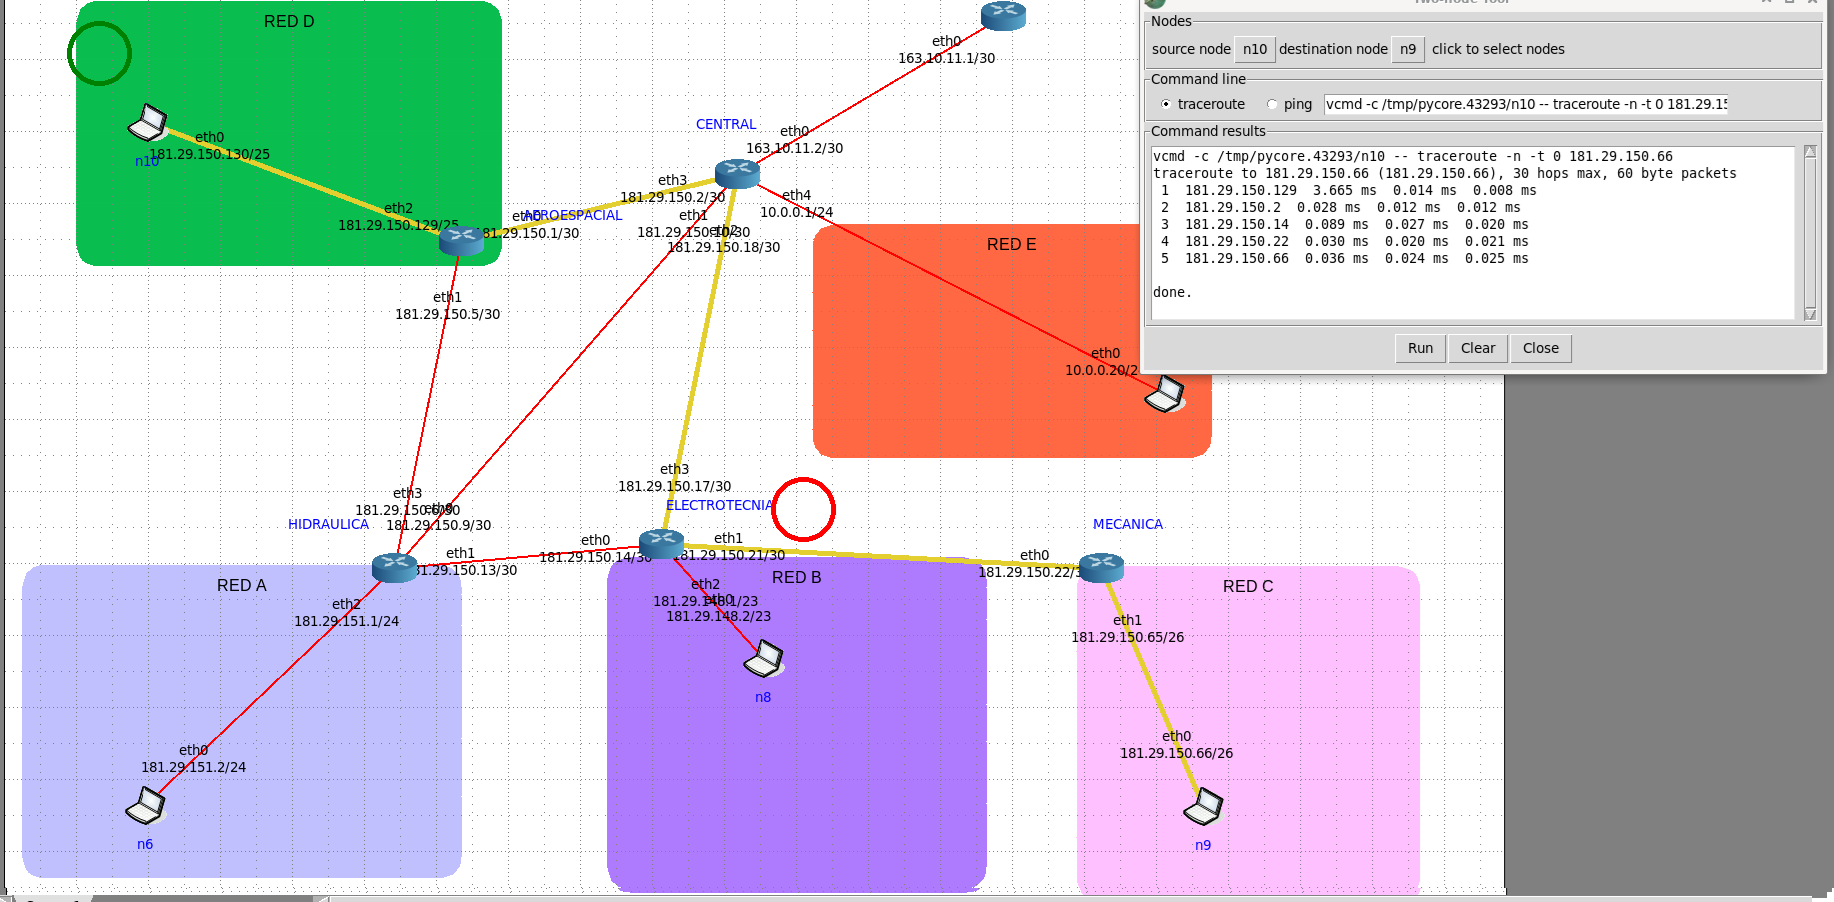
\includegraphics[width=0.43\textwidth]{./Imagenes/traceroute_4.png}
	\caption{Traceroute desde n10 a n9}
\end{figure}

Para corroborar que los dispositivos tuvieran conexión a internet se hizo \textit{traceroute} de los diferentes dispositivos a la IP \textit{163.10.11.1} (ISP).

\textit{En la realidad habría que hacer un ping o traceroute a la dirección 8.8.8.8 por ejemplo, o alguna conocida como google.com.ar. Pero en este caso se simula que la conexión a internet está hecha cuando se pueden dirigir paquetes al ISP.}

También sería necesario implementar un NAT\footnote{NAT (Network Address Translation) es una técnica utilizada en redes para modificar las direcciones IP en los paquetes de datos que pasan a través de un router o firewall. Permite que múltiples dispositivos en una red local (LAN) compartan una única dirección IP pública, facilitando la conservación de direcciones IPv4 y añadiendo una capa de seguridad al ocultar las direcciones internas de los dispositivos.} en el \textit{router central} o en el \textit{router del ISP} para enmascarar las IPs privadas. Sin embargo, si se tuviera que implementar en un escenario real, no sería posible hacerlo en el \textit{router del ISP} debido a la falta de acceso, por lo que únicamente podría realizarse en el \textit{router central}.

\section{Implementación del servidor TCP}

El protocolo TCP descompone los datos en paquetes y los reenvía a la capa del protocolo de Internet (IP) para garantizar que cada mensaje llegue a su ordenador de destino. El estado actual de desarrollo del protocolo TCP permite establecer una conexión entre dos puntos terminales en una red informática común que posibilite un intercambio mutuo de datos. En este proceso, cualquier pérdida de datos se detecta y resuelve, por lo que se considera un protocolo fiable. La secuencia específica para establecer una conexión con el protocolo TCP es la siguiente:

\begin{enumerate}
	\item En el primer paso, el cliente que desea establecer la conexión envía al servidor un paquete SYN o segmento SYN (del inglés synchronize = “sincronizar”) con un número de secuencia individual y aleatorio. Este número garantiza la transmisión completa en el orden correcto (sin duplicados).
	\item Si el servidor ha recibido el segmento, confirma el establecimiento de la conexión mediante el envío de un paquete SYN-ACK (del inglés acknowledgement = “confirmación”) incluido el número de secuencia del cliente después de sumarle 1. De forma adicional, transmite un número de secuencia propio al cliente.
	\item Para finalizar, el cliente confirma la recepción del segmento SYN-ACK mediante el envío de un paquete ACK propio, que en este caso cuenta con el número de secuencia del servidor después de sumarle 1. En este punto también puede transmitir ya los primeros datos al servidor.
\end{enumerate}

\begin{figure}[H]
	\centering
	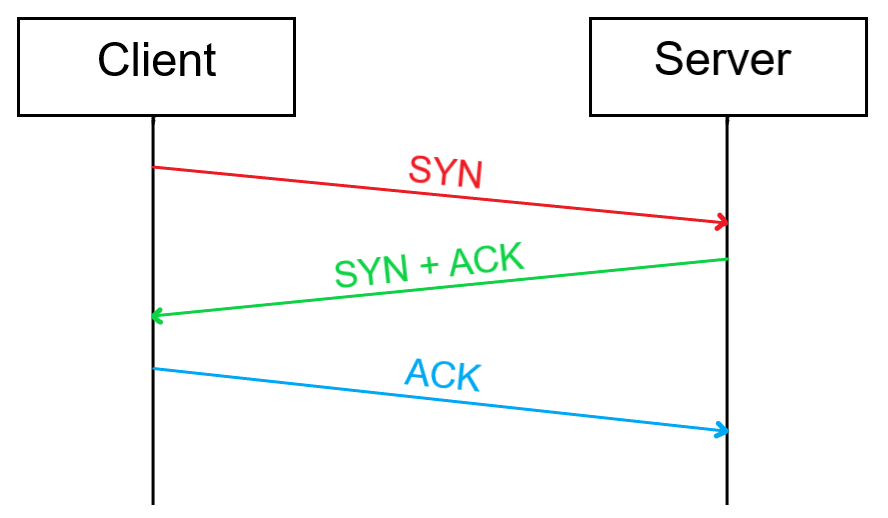
\includegraphics[width=0.43\textwidth]{./Imagenes/tcp_ack.png}
	\caption{Diagrama de la sincronización del TCP}
	\label{fig:tcp_ack}
\end{figure}

\subsection{Cabecera TCP}

\begin{figure}[H]
	\centering
	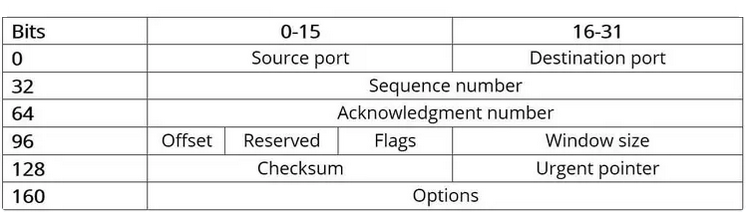
\includegraphics[width=0.43\textwidth]{./Imagenes/TPC_header.png}
	\caption{Estructura de la cabecera TCP}
	\label{fig:tcp_header}
\end{figure}

\subsection{Lógica del código}

\begin{figure}[H]
	\centering
	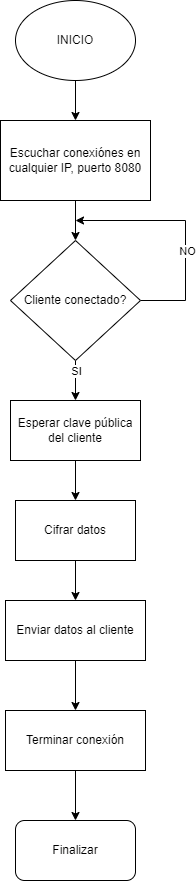
\includegraphics[height=270pt]{./Imagenes/diagrama_flujo_server.png}
	\caption{Diagrama de flujo del servidor}
	\label{fig:flujo_server}
\end{figure}

\begin{figure}[H]
	\centering
	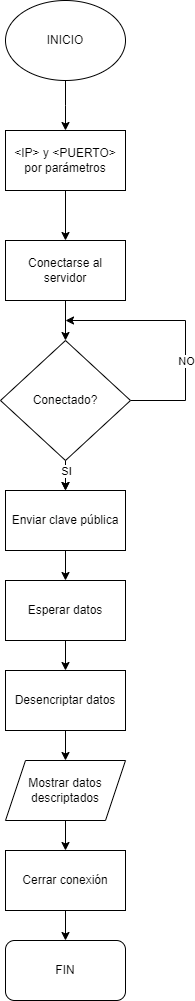
\includegraphics[height=270pt]{./Imagenes/diag_flujo_cliente.png}
	\caption{Diagrama de flujo del cliente}
	\label{fig:flujo_cliente}
\end{figure}

Los diagramas \ref{fig:flujo_cliente} y \ref{fig:flujo_server} explican el comportamiente general de ambos programas. Las principales características son:

\subsubsection{Cliente}
\begin{itemize}
	\item Debe recibir como parámetro la \textbf{IP} y el \textbf{puerto} del servidor para conectarse.
	\item Debe \textbf{enviar} la clave pública de encriptación.
	\item Imprime los datos desencriptados en pantalla.
\end{itemize}

\subsubsection{Server}
\begin{itemize}
	\item El puerto por defecto es \textbf{8080}.
	\item Debe \textbf{recibir} la clave pública de encriptación.
	\item Enviar los datos encriptados con la llave pública.
\end{itemize}

\textit{En los códigos se pueden habilitar los comentarios de debugeo descomentando el macro DEBUG. Para recompilar los códigos se puede emplear el Makefile, corriendo: make client y make server.}

\subsection{Capturas de paquetes con Wireshark}

Se ejecutó el servidor en el dispositvo \textbf{n6} (\textit{181.29.150.2}) y el cliente en el dispositvo \textbf{n10} (\textit{181.29.150.130}), y con Wireshark\footnote{Wireshark es un analizador de protocolos de red de código abierto que permite capturar y examinar en detalle el tráfico de datos en una red en tiempo real. Es ampliamente utilizado en la industria para diagnóstico de problemas, desarrollo de software y aprendizaje de protocolos de comunicación.} se hizo la captura de los paquetes en el cliente. En las siguientes figuras se muestra como se capturan los datos, además se puede ver como se hace la conexión TCP como se explicó en \ref{fig:tcp_ack}.

\begin{figure}[H]
	\centering
	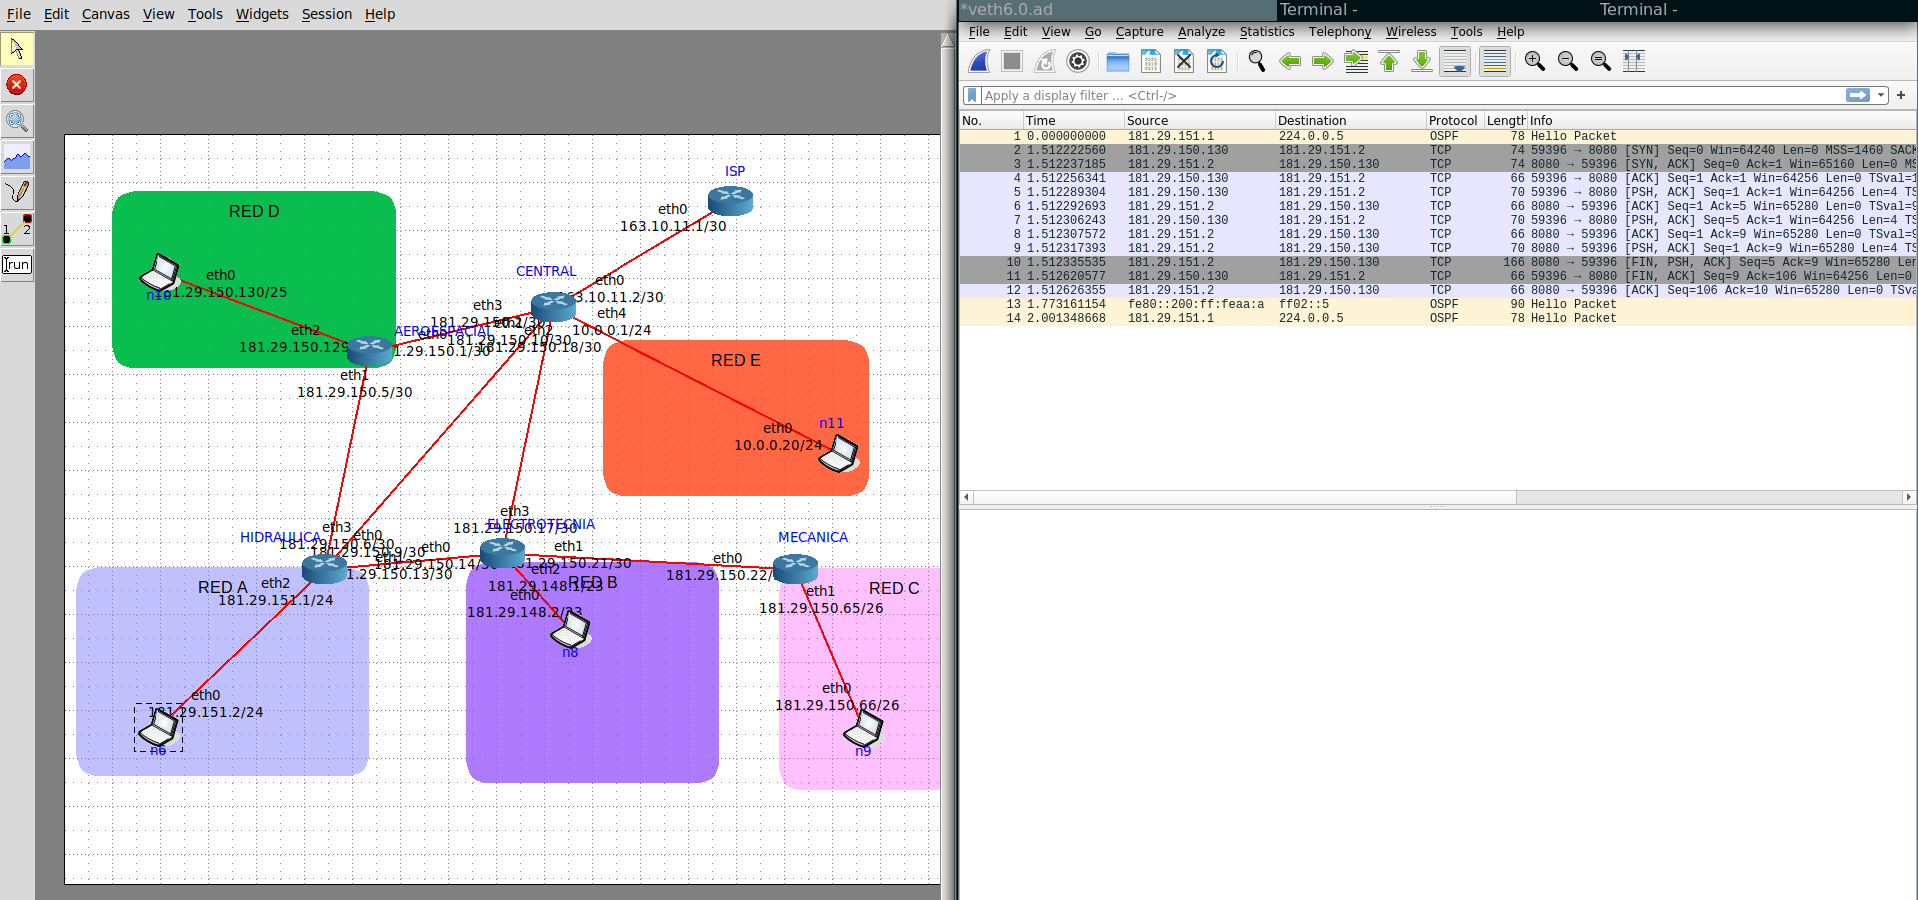
\includegraphics[width=0.43\textwidth]{./Imagenes/captura_wireshark_n6_n10.png}
	\caption{Trafico entre \textbf{n6} y \textbf{n10}}
	\label{fig:wireshark_n6_n10}
\end{figure}

\begin{figure}[H]
	\centering
	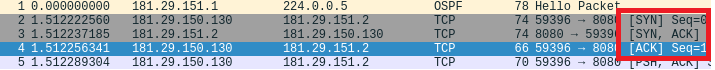
\includegraphics[width=0.43\textwidth]{./Imagenes/trafico0.png}
	\caption{Trafico entre \textbf{n6} y \textbf{n10}, TCP}
	\label{fig:wireshark_0}
\end{figure}

\begin{figure}[H]
	\centering
	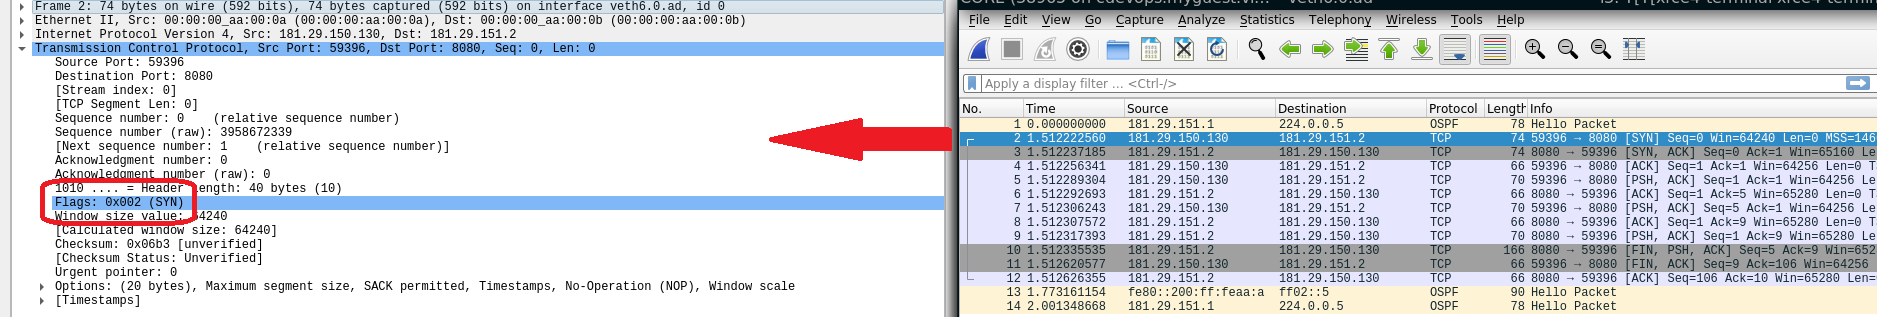
\includegraphics[width=0.43\textwidth]{./Imagenes/trafico1.png}
	\caption{Trafico entre \textbf{n6} y \textbf{n10}, TCP SYN}
	\label{fig:wireshark_1}
\end{figure}

\begin{figure}[H]
	\centering
	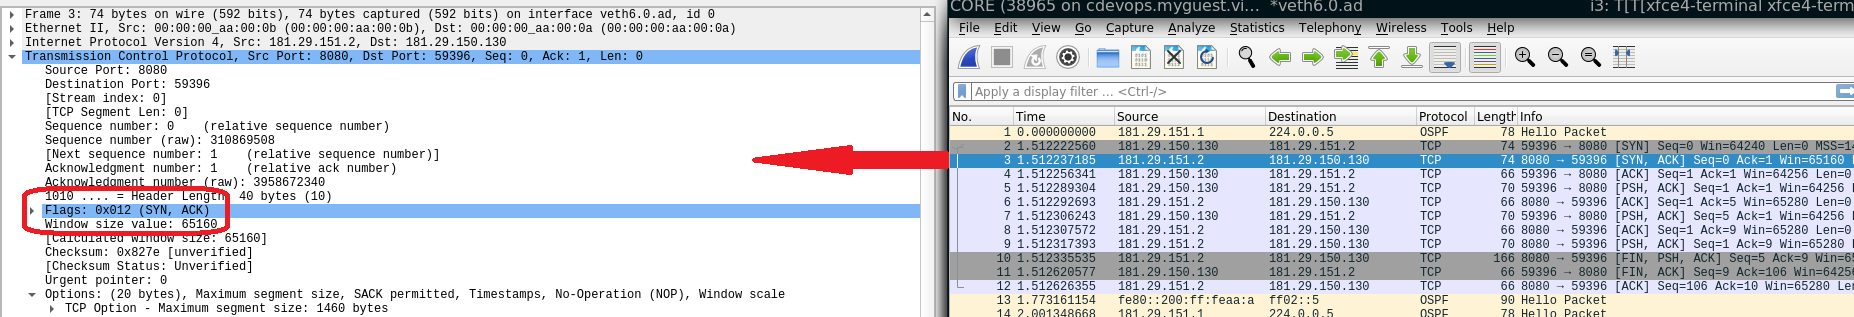
\includegraphics[width=0.43\textwidth]{./Imagenes/trafico2.png}
	\caption{Trafico entre \textbf{n6} y \textbf{n10}, TCP SYN-ACK}
	\label{fig:wireshark_2}
\end{figure}

\begin{figure}[H]
	\centering
	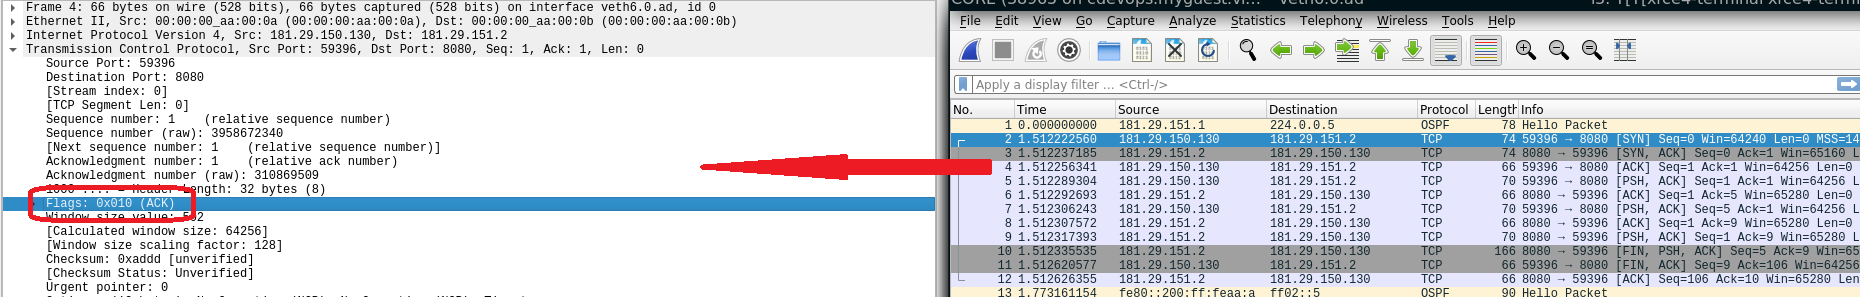
\includegraphics[width=0.43\textwidth]{./Imagenes/trafico3.png}
	\caption{Trafico entre \textbf{n6} y \textbf{n10}, TCP ACK}
	\label{fig:wireshark_3}
\end{figure}

A continuación, se muestran los paquetes que contienen los datos. En la figura \ref{fig:wireshark_4} se observa que la bandera PUSH está en 1, lo que indica que la transmisión se realiza de un dato (número) a la vez. También se puede notar que la transmisión es del cliente al servidor, ya que dicho dato corresponde a la clave pública. Posteriormente, en la figura 18 se muestra cómo el TCP Segment Len es distinto de 0, ya que se están transmitiendo datos. Este paquete en particular corresponde a uno de los números encriptados que el servidor transmite. 

\begin{figure}[H]
	\centering
	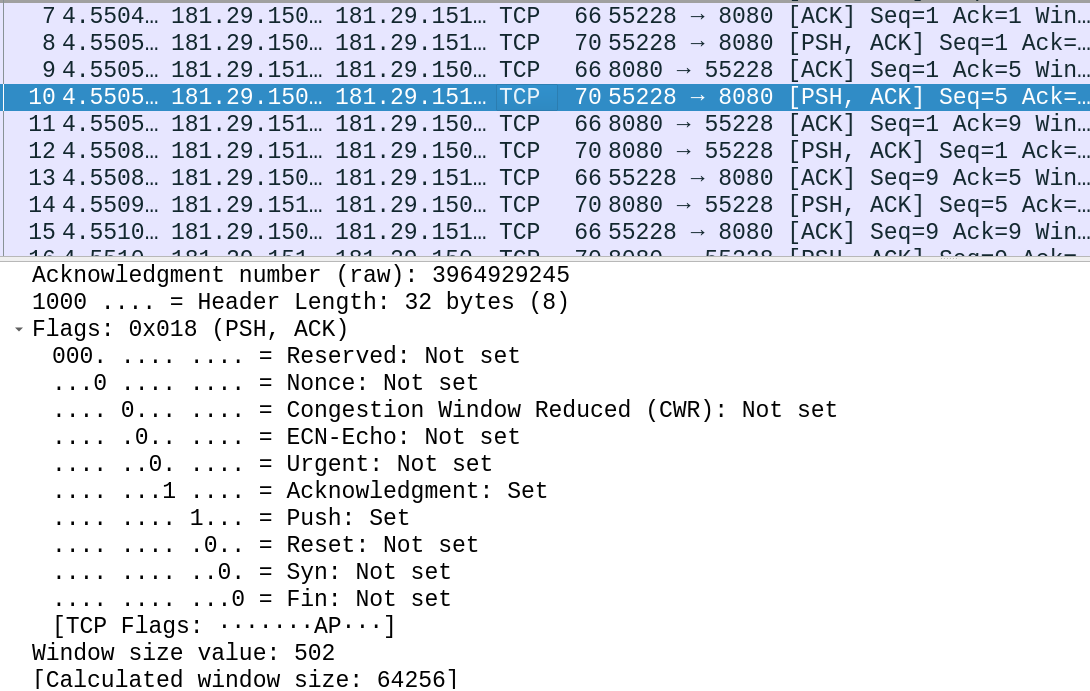
\includegraphics[width=0.43\textwidth]{./Imagenes/tcp_datos_1.png}
	\caption{Trafico entre \textbf{n6} y \textbf{n10}}
	\label{fig:wireshark_4}
\end{figure}

\begin{figure}[H]
	\centering
	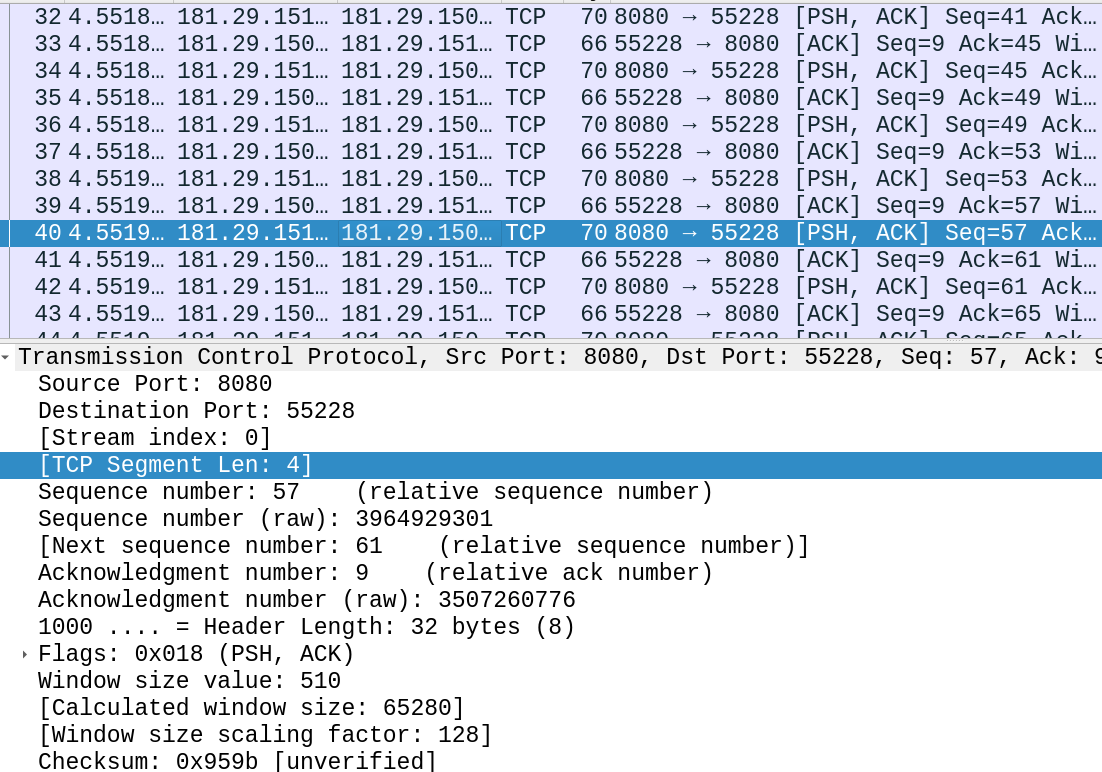
\includegraphics[width=0.43\textwidth]{./Imagenes/tcp_datos_2.png}
	\caption{Trafico entre \textbf{n6} y \textbf{n10}}
	\label{fig:wireshark_5}
\end{figure}

\subsection{Archivos}

Junto al presente se adjuntan las imágenes para que el lector las pueda ver con más detalle, además se encuentra un archivo (``core.txt'') que contiene los datos sobre el enrutamiento de la topología dada.

\end{document}